%%%%%%%%%%%%%%%%%%%%%%% file template.tex %%%%%%%%%%%%%%%%%%%%%%%%%
%
% This is a general template file for the LaTeX package SVJour3
% for Springer journals.          Springer Heidelberg 2010/09/16
%
% Copy it to a new file with a new name and use it as the basis
% for your article. Delete % signs as needed.
%
% This template includes a few options for different layouts and
% content for various journals. Please consult a previous issue of
% your journal as needed.
%
%%%%%%%%%%%%%%%%%%%%%%%%%%%%%%%%%%%%%%%%%%%%%%%%%%%%%%%%%%%%%%%%%%%
%
% First comes an example EPS file -- just ignore it and
% proceed on the \documentclass line
% your LaTeX will extract the file if required
\begin{filecontents*}{example.eps}
%!PS-Adobe-3.0 EPSF-3.0
%%BoundingBox: 19 19 221 221
%%CreationDate: Mon Sep 29 1997
%%Creator: programmed by hand (JK)
%%EndComments

\end{filecontents*}
%
\RequirePackage{fix-cm}
%
\documentclass[final]{svjour3}                     % onecolumn (standard format)
%\documentclass[smallcondensed]{svjour3}     % onecolumn (ditto)
%\documentclass[smallextended]{svjour3}       % onecolumn (second format)
%\documentclass[twocolumn]{svjour3}          % twocolumn
%
\smartqed  % flush right qed marks, e.g. at end of proof
%
\usepackage[authoryear,comma]{natbib}
 \usepackage{mathptmx}      % use Times fonts if available on your TeX system
%
% insert here the call for the packages your document requires
\usepackage[pagebackref=true,colorlinks=true, linkcolor=blue,anchorcolor=blue,citecolor=blue,filecolor=blue,menucolor=blue,
urlcolor=cyan,plainpages=false,pdfpagemode=UseThumbs,pdftitle={Titre},pdfauthor={oluwole},
pdfsubject={Thesis},pdfstartview=FitH]{hyperref}% Extensions PDF
%\def\pdfBorderAttrs{/Border [0 0 0] } % Options PDF (No border around Links)
%\usepackage[plainpages=false,backref=page,hypertexnames=true,linktocpage=true,colorlinks=true,citecolor=blue,linkcolor=blue]{hyperref}
\usepackage{pdfpages}
%\usepackage{chicago}
\usepackage[onehalfspacing]{setspace}
%\doublespacing
%\linespread{1.6}
\setstretch{1.5}
\usepackage{apalike}
\onehalfspacing
\usepackage[left=40mm,right=25mm,top=30mm,bottom=20mm,headsep=10mm]{geometry}
\geometry{a4paper}
%\usepackage{amsmath}

\usepackage{amsmath,amsfonts,amssymb}

\usepackage{fancybox}
\usepackage{graphicx}
\usepackage{setspace}
\usepackage[small]{caption}
\usepackage{color}
\usepackage{placeins}
\usepackage{epstopdf}
\usepackage{booktabs}
\usepackage{tikz}
\usepackage{subcaption}
%
% please place your own definitions here and don't use \def but
% \newcommand{}{}
%
 %Oluwole
 
\DeclareMathSymbol{\bLambda}{\mathalpha}{letters}{"03}
%\DeclareMathSymbol{\bGamma}{\mathalpha}{letters}{"00}
%\DeclareMathSymbol{\hbGamma}{\mathalpha}{letters}{"00}

\newcommand{\bt}{{\bf t}}
\newcommand{\bB}{{\bf B}}
%\newcommand{\Sigma}{{\bf \Sigma}}
\newcommand{\tbSigma}{{\tilde {\bf \Sigma}}}
\newcommand{\tbu}{{\tilde {\bf u}}}
\newcommand{\tbU}{{\tilde {\bf U}}}
\newcommand{\bh}{{\bf h}}
\newcommand{\bH}{{\bf H}}
\newcommand{\bD}{{\bf D}}
\newcommand{\bU}{{\bf U}}
\newcommand{\bu}{{\bf u}}
\newcommand{\bZ}{{\bf Z}}
\newcommand{\bz}{{\bf z}}
\newcommand{\bC}{{\bf C}}
\newcommand{\bc}{{\bf c}}
%%
\newcommand{\bx}{{\bf x}}
\newcommand{\bX}{{\bf X}}
\newcommand{\by}{{\bf y}}
\newcommand{\bY}{{\bf Y}}
\newcommand{\bE}{{\bf E}}
\newcommand{\bW}{{\bf W}}
\newcommand{\tbx}{{\tilde {\bf x}}}
\newcommand{\tbX}{{\tilde {\bf X}}}
\newcommand{\tby}{{\tilde {\bf y}}}
\newcommand{\tbY}{{\tilde {\bf Y}}}
\newcommand{\hbX}{{\hat {\bf X}}}
\newcommand{\hbY}{{\hat {\bf Y}}}
\newcommand{\hby}{{\hat {\bf y}}}
\newcommand{\ty}{{\tilde {y}}}
\newcommand{\hy}{{\hat {y}}}

%%%%%%Upper
\newcommand{\bGamma}{{\boldsymbol{\Gamma}}}
\newcommand{\tbGamma}{{\tilde{\boldsymbol{\Gamma}}}}
\newcommand{\hbGamma}{{\hat{\boldsymbol{\Gamma}}}}

%%%%%%%Lower
\newcommand{\bgamma}{{\boldsymbol{\gamma}}}
\newcommand{\bepsilon}{{\boldsymbol{\varepsilon}}}
\newcommand{\tbepsilon}{{\tilde{\boldsymbol{\varepsilon}}}}
\newcommand{\hbepsilon}{{\hat{\boldsymbol{\varepsilon}}}}
\newcommand{\bbeta}{{\boldsymbol{\beta}}}
\newcommand{\hbbeta}{{\hat{\boldsymbol{\beta}}}}
\renewcommand{\epsilon}{\varepsilon}
%%%%%%%%%%%









%==========Divers===========:
\DeclareMathOperator*{\ssum}{{\textstyle \sum}}

% Insert the name of "your journal" with
 \journalname{Environmental and Ecological Statistics}

%
\begin{document}
%
\title{Bayesian emulation of climate change impact on crop yields%\thanks{Grants or other notes
%about the article that should go on the front page should be
%placed here. General acknowledgments should be placed at the end of the article.}
}
%\subtitle{Do you have a subtitle?\\ If so, write it here}

\titlerunning{Bayesian emulation of climate change impact on crop yields}        % if too long for running head

\author{Oluwole K. Oyebamiji  \and Neil R. Edwards  \and
Philip B. Holden  \and 
Paul H. Garthwaite  \and
Sibyll Schaphoff  \and
         Dieter Gerten
}

%\authorrunning{Short form of author list} % if too long for running head

\institute{The Open University, Environment, Earth \& Ecosystems \at Milton Keynes, MK7 6AA, UK. \\
              Tel.: (+44) 7411875750\\
              Fax: (+44) 1908 655 151\\
              \email{wolemi2@yahoo.com}           %  \\
%             \emph{Present address:} of F. Author\\
\and Neil R. Edwards  \and Philip B. Holden \\ 
The Open University, Environment, Earth \& Ecosystems, Milton Keynes, UK
  %  if needed
           \and
           %S. Author \at
\\ P.H. Garthwaite\\
              %second address
Department of Mathematics \& Statistics,
 The Open University,
Milton Keynes,
UK
\and
\\
S. Schaphoff  \and D. Gerten\\
Potsdam Institute for Climate Impact Research (PIK),
 Telegrafenberg A62,
14473 Potsdam,
Germany
}

\date{Received: date / Accepted: date}
% The correct dates will be entered by the editor


\maketitle

\begin{abstract}
The global climate is changing and this has a great negative impact on ecosystems. It adversely affects the environment, life quality, the economy, agriculture. Assessment of future climate change on agricultural productivity is attracting increasing attention among the modellers, since modelling provides a thorough way of quantifying the crop yield response under climate uncertainty. Adequate knowledge of the impacts of climate change on agricultural crop is required to fully understand global food security. In order to address this problem, the common tradition is to run a high complex process-based simulation models. This assessment is challenging because the models are computationally intensive and simulation runs are often limited. This problem can be eradicated by using a statistical approximation of the complex models which will help in reducing the computational burden. Our aim in this paper is to build a cheaper surrogate models (called emulators) from simulations of the LPJmL dynamic global vegetation and crop model. The paper focuses on global predictions of crop yield change with their associated uncertainty levels. We proposed a two-stage approach where we used a stepwise regression in the first stage  and combined both principal component analysis and Bayesian technique for residual interpolation in stage 2. %We first applied a linear regression to the multi-dimensional and high spatial resolution data. This will capture most of the spatial and temporal variability. The residuals obtained from this regression results are aggregated to a country level and modelled by a GP regression. %The explanatory variables for the GP regression is provided by predictions obtained from regression results are decomposed by PCA to reduce the dimension of the data. 

\keywords{Bayesian techniques \and GP emulator \and stepwise regression \and PCA \and LPJmLem \and crop yields}
\end{abstract}

%\section{Introduction}

\section{Introduction}
The global climate is changing and this has a great negative impact on ecosystems. It adversely affects the environment, life quality, the economy and  agriculture. Any change in the climate system over time, whether due to natural variability or human activity, is referred to as climate change \citep{42}. Of a particular priority in this paper is the assessment of the impacts of future climate change on terrestrial ecosystems. Assessment of climatic impacts on global vegetation is attracting increasing attention among modellers, since modelling provides a thorough way of quantifying the biospheric response under climate uncertainty. Adequate knowledge of the impacts of climate change on agricultural crops is required to fully understand global food security.
Future increases in the demand for food and reduced availability of land for growing pose major challenges for human society as a result of rising projections for world population over the next century.
Growth in demand for food will also put pressure on water resources. Rising temperature, CO$_2$ emissions and associated climate change will affect global food and water supplies. Potential climatic impacts on vulnerable populations through lack of adequate food and regular water supply have been identified as other serious threats. 
\citet{ipc14} reported that for the major crops (wheat, rice, and maize) in tropical and temperate regions, climate change without adaptation will negatively impact production for local temperature increases of $2^{\circ}C$ or more above late-20th-century levels, although individual locations may benefit with medium confidence.

Modelling tools for studying the interaction between climate change and its effects are relatively under-developed. In spite of tremendous progress in the statistical analysis of climate change studies, quantifying the climatic impact on agricultural crops still suffer problems. In addition, adequate knowledge of climatic impacts on agricultural productivity is essential. For instance, comprehensive and detailed understanding of the impact of climate change on global crop yields is required for maintaining good management practices for sustainable agriculture. However, this assessment is challenging and computationally intensive models have to be run. 

The Lund-Potsdam-Jena-managed Land (LPJmL) model is a process-based dynamic global vegetation and crop model. The global responses of carbon and vegetation patterns under climate change for both natural and agricultural ecosystems can be simulated by LPJmL. The model is used in this study to simulate the response of terrestrial ecosystems to climate change. The run times for LPJmL are high and this often makes the full assessment of the impact of climate change on the ecosystems impossible. Both statistical and process-based models have been used extensively since fourth assessment results AR4 to assess the response of crop yield to temperature \citep{ipc14}.
Statistical emulation can help to overcome this problem. Emulation integrates both the process-based model and statistical techniques. Besides, emulators offer rapid and relatively quick alternatives for projection of climate change impacts on agricultural productivity for diverse climate scenarios \citep{qwole}. For instance, \cite{q101,q102} considered both economic and physically based modelling approaches to project global and regional impact of climate change, but due to computing constraints only a limited set of scenarios were investigated. Another benefit of emulation is the provision of a measure of uncertainties associated with the projections. 


Several techniques have been used for modelling effect of climate and weather on crop yield. 
\citet{r5} compared the predictive performance of stepwise multiple linear regression with that of projection pursuit regression. In related studies, \citet{r6} and \citet{r8} considered multiple linear regression techniques using polynomial and interaction terms for modelling crop productivity measure. In contrast to the regression approaches of \citet{r26,r6,r9},  \citet{r30} and \citet{r29} applied a non-parametric approach to crop yield prediction. \citet{r23} applied a Bayesian bootstrap method to similar data.

\cite{91,89} proposed a Bayesian statistical model that combines information from a multi-model ensemble of Atmospheric Ocean General Circulation Models (AOGCMs) with observations in order to determine the probability distribution of future climate change. A probabilistic method to overcome the challenge of inclusion of model inadequacy in order to improve the quality of a simulator ensemble was presented in \citet{46} and in \citet{68}. \citet{32} estimated the uncertainty associated with the carbon flux simulated from a dynamic global vegetation model. They used a GP emulation technique proposed by \cite{60} to quantify these uncertainties for England and Wales.

Similarly, \cite{q23} applied the \cite{60} approach in conjunction with a PCA for basis representations of high-dimensional output. Apart from reducing the dimensionality of the problem this PCA technique also reduces the computation time required for obtaining the posterior distributions. A closely related study of \cite{80} performed a calibration of multivariate experiments by extending the approach of \cite{45} to multivariate models. This study incorporated principal component analysis, like \cite{q23}, to project the multivariate output to a lower subspace. \cite{10} focuses on variety of dimension reduction methods. 
 
\cite{83} described the behaviour of large linear dynamic models using statistical principles of dynamic emulation. Their approach identifies a low-order model that approximates the behaviour of the high-order dynamic simulator that is much cheaper. \cite{q5} described a Bayesian method for quantification of uncertainty in complex computer models. \cite{q17} described some notable examples where GP modelling applications have been implemented. \citet{q22} and \citet{q23} applied a principal component to decompose and emulate multivariate responses. The goal of this paper is to assess the global impact of climate change on agricultural crops and to provide measure of uncertainty associated with the projections.

We propose a two-stage approach where we use a stepwise regression in the stage 1  and combined both principal component analysis and Bayesian techniques for residual interpolation in the stage 2. We first apply a linear regression to the multi-dimensional and high spatial resolution data. This captures most of the spatial and temporal variability. The residuals obtained from stage 1 results are aggregated to a country level and modelled by a combination of PCA and GP regression. In the second stage, we use a GP regression for emulation of unexplained residual. The final results are then compared with \citet{qwole} approach that demonstrated a weighted least regression using different distance metrics for residual interpolation.

We describe the models and simulation data used for the analysis in Section 2. In Section 3 we describe the methods and emulation procedures. Section 4 provides the results of the analysis. Sections 5 and 6 present the discussion and concluding comments respectively.

\section{Models and data}
%\subsection{Models used for the analysis}
The data used for this study are provided by the LPJmL and Spatial Climate Generator (ClimGEN).
%MAGICC is a simple carbon cycle climate model that simulates greenhouse gas (GHG) cycles, radiative forcing, and ice melt. MAGICC6 is a new version of MAGICC \cite{54} and is able to simulate global mean temperature (GMT) trajectories based on the emulation of the 18 Atmospheric Ocean General Circulation Models (AOGCMs) used in \cite{92} for the Fourth Intergovernmental Panel on Climate Change (IPCC) assessment report. ClimGen is a spatial climate scenario generator. 
The LPJmL model of \cite{8} is a dynamic global vegetation model \cite{r34} enhanced to represent global agriculture in addition to natural vegetation. Agricultural productivity is simulated through varieties of crop functional types (CFTs), both rainfed and irrigated. The LPJmL model takes as inputs climate variables such as precipitation, temperature and insolation, which are then disaggregated to quasi-daily values by a weather generator. The monthly input and output data are spatially explicit time series of about 60 000 global $0.5^{\circ}$ resolution grid cells. ClimGEN emulates the spatial response patterns by disaggregating the temperature trajectories to $0.5^{\circ}$ spatial resolution of climate change patterns for temperature, precipitation and cloud cover. The generated climate scenarios are supplied as inputs to run the LPJmL simulation for the assessment of climate impacts on variables such as potential crop yield.

\subsection{Simulation data}\label{data2}
The input data are monthly climate variables (temperature, precipitation, cloud cover and wetday frequency) from ClimGEN. All the simulation data are on a global $0.5^{\circ} \times 0.5^{\circ}$ degrees resolution. The data cover a period of $2001-2100$. There are seven different General Circulation Models (GCMs) and each is applied to 4 RCPs, giving a total of 28 different climate scenarios. The other inputs are annual CO$_2$ concentrations for all the 4 RCPs, soil data that describes 8 different soil types.

The output data from LPJmL are potential crop yields. The crop yields are annual values for 12 CFTs, with rainfed and irrigated outputs considered separately. We have chosen only 4 CFTs namely temperate cereal, rice, maize and oil, (oil crop is a combination of sunflower, soyabean and rapeseed) for emulation. In addition, the crop yields have 7 seven different crop management levels for each scenario, and performed simulations with and without CO$_2$ fertilization effect. In calibrating crop management, the Leaf Area Index (LAI) is a key parameter. LAI is the ratio of total upper leaf surface of vegetation divided by the surface area of the land on which it grows. Crop management levels are represented by maximum leaf area index LAI$_{max}$, further descriptions of the data used for this analysis are documented in \cite{qwole}.


\section{Methods}
 A Bayesian framework for emulation is almost always based on the assumption that a Gaussian process prior distribution can be specified for unknown parameters and hyperparameters.  Under a Bayesian perspective unknown parameters are treated as random variables. The given prior distribution can be updated from training data. Applying Bayes rule to this setting, a posterior distribution can be obtained. The posterior distribution is also a Gaussian process. 

A major difficulty with GP modelling is the computational effort associated with dealing with large data, as computer time scales are of order $O(n^3)$ where $n$ is the number of observations. Several techniques have been adopted to overcome this computational problem. Earlier techniques are documented in \citet{q10} and \cite{q47}. In particular, \cite{q18} used hierarchical Gaussian process mixtures for regression of a large dataset with repeated measurements. 
GP emulation is based on the Bayesian technique and experimental design of computer experiments for predicting model outputs at test input point \citet{q7} and \citet{70}. A GP emulator assumes that a simulator output is an unknown function $g(.)$. We can then choose a prior distribution for $g(.)$ using the Bayesian approach and update this distribution, with some data obtained from the simulator runs.

There are several techniques for estimating hyperparameters of the GP model. Analytical estimates of the hyperparameters of $\boldsymbol \beta$ and $\sigma^2$ in this paper are derived by integrating out the nuisance parameters as discussed in next section. We apply the MLE technique for the estimation of correlation $\rho$ hyperparameter also described in Appendix 1. Maximum likelihood is computationally feasible and depends on the assumption of multivariate Gaussian distribution.
In this paper, we analyse the crop yield data using Bayesian techniques. We are implementing a Bayesian technique because of its wide applicability and flexibility. Another additional benefit of Bayesian modelling is the quantification of the model uncertainty.

The motivation for this paper is to demonstrate the concept of GP regression in modelling crop yield data and to compare the results with some existing techniques. In particular, we demonstrate combinations of stepwise regression, PCA and GP techniques in emulating the crop yield response under global climate scenarios. We examine whether the non-parametric modelling of the unexplained residual using Gaussian process (GP) in the second stage provides a useful result. LPJmL simulation runs are computationally expensive and to reduce this high computational cost we describe the statistical emulation of LPJmL crop outputs in this paper, where a two-stage technique was proposed. In the stage 1, stepwise regression was applied onto crop yield, and a GP regression was used for residual interpolation in the stage 2. 

A Gaussian process model could not be applied directly to the stage 1 because of the computational difficulty in the sample size coupled with the large number of parameters to be estimated. GP scales cubically with the number of observations $O(N^3)$, which is not appropriate for our present data, even after averaging decadally and sampling from each scenario. The data matrix contains over 4.5 million observations. It is possible to use GP for residual interpolation. However, this approach still has a high computational cost, and it is necessary to reduce the spatial resolution and aggregate data to a country level in order to reduce the computational load. Our procedure is described below. 

\subsection{Emulation procedure}
The emulators were constructed in two stages. Our objective is to produce a statistical approximation that will link the model climate inputs $\textbf X$ to the deterministic vector outputs $\by$ from LPJmL. Let the relationship between the climate input data from ClimGen and each output from LPJmL be represented by a model
%$$\by=f(\textbf X) + \boldsymbol\varepsilon,$$ 
\begin{equation}\label{geneq}
y=f(\textbf{X})+\boldsymbol\varepsilon= \boldsymbol\beta_0+\boldsymbol\beta_{1}x_{1}+\ldots +\boldsymbol\beta_{p}x_{p}+ \boldsymbol\beta_{1}x_{1,1}^{2}+\ldots+\boldsymbol\beta_{p}x_{p,p}^2+\boldsymbol\beta_{1,2}x_{1}x_{2}+\dots +\boldsymbol\beta_{(p-1),p}x_{(p-1)}x_{p}+\boldsymbol\varepsilon
\end{equation}
where $\by$ is the (vector) simulated mean decadal change for LPJmL crop-yield over the grid cells for all scenarios, $\boldsymbol \varepsilon$ represents all the unexplained variation in $f(\textbf X)$ which is not captured by the stepwise regression method in stage 1. Values of $\boldsymbol \varepsilon$ are spatially correlated for scenarios that are very close in the input space. In the second stage, we model $\boldsymbol \varepsilon$ as a Gaussian random process with unknown mean and covariance functions. GP is an extension of multivariate Gaussian distributions to infinite dimensionality with associated mean and covariance matrix.

\subsubsection{Stage 1}
The LPJmL crop-yield data were based on simulations for 59199 grid cells on $0.5^{\circ}$ by $0.5^{\circ}$, but here we only focused on current crop growing areas (the other cells are truncated).
We built separate emulators for the rainfed and irrigated crops. Four crops were selected for emulation; temperate cereal, rice, maize and oil crop. The oil crop is a maximum yield among soybean, sunflower and rapeseed. 
The average decadal yield given by LPJmL from 2005-2095 was computed for each crop and each scenario. We then obtained the change in yields relative to the baseline values. Baseline values are the average decadal yield of LPJmL outputs and climate data for the period 2005-2014, and are used as a reference for computing the relative change in yields and climate. We calculated the change in seasonal climate variables for the input variables listed in Table \ref{tt1}. Baseline yields, baseline seasonal climate and change in seasonal climate variables are used as input to the first stage emulator. CO$_2$, latitude, soil type and $LAI_{max}$ are also included as additional inputs. We produce different emulators for irrigated and rainfed crops but combine the entire scenario together.

The emulators were built from two GCMs with relatively moderate equilibrium climate sensitivity, CCCMA-CGCM31 and CCSR-MIROC32HI, four RCPs, and two simulation categories (with and without CO$_2$ fertilization effect), giving 16 different scenarios. Each scenario has seven crop management levels and eight time-slices, with each time-slice consisting of 16 649, 6913, 19 139 and 8427 valid grid points per scenario for rainfed temperate cereal, rice, maize and oil, respectively, and 8963, 7325, 9146 and 2731 for irrigated crops. Another five GCMs, UKMO-HADGEM1, GISS-MODELER, GISS-MODELEH, IPSL-CM4 and CCSR-MIROC32MED were selected for cross-validation purposes. 

We use observations from 5000 randomly sampled grid points because the stepwise algorithm could not handle the whole dataset. The 5000 grid points are fixed across the time-slice, RCP, GCM and management levels as well as simulation categories and similarly in each of 37 input variables (see Table \ref{tt1}) in Appendix. Irrigated oil has less than 5000 observations so we used all the simulation data. We then fitted a stepwise regression model (including linear, quadratic and all two-way interactions) to the sampled data for each change in crop-yield when crops are rainfed. This procedure was carried out for each of the four crops and repeated for the case where crops are irrigated. Further details of this procedure are given in \citep{qwole}.


\subsubsection{Stage 2}
Consider a single crop/irrigation regime/management level/time slice combination and let $\by_{i}$ be the vector of changes in yield given by LPJmL for that combination in the $i^{th}$ scenario ($i=1,\ldots,16$). We let $\tby_{i}$ be the corresponding predictions given by the stage 1 emulator and $\bepsilon_i = \by_{i} - \tby_{i} $ is the error in prediction. Each $\tby_{i}$ and $\bepsilon_i$ is an $N\times 1$ vector, where $N$ denotes the number of grid cells for that crop/irrigation regime. As $\tby_{1},\ldots, \tby_{16}$ are predictions on {\em training} data, the values of $\bepsilon_1,\ldots,\bepsilon_{16}$ are known.

Given a new vector of predictions, $\tby^{new}$, from a new scenario where the emulator values are unknown, the aim is to estimate the error of $\tby^{new}$ from $\bE=(\bepsilon_1,\ldots,\bepsilon_{16})$ and $\tbY=(\tby_1,\ldots, \tby_{16})$ denoted as  $\bepsilon^{new}$.
In order to reduce the dimension of prediction data from stage 1 emulator, we apply a PC decomposition to the $16\times N$ matrix $\tbY^{\rm T}$, and select just the first four principal components. The resulting $16\times 4$ matrix of PC scores given by these four components is denoted as $\bU$. The columns of a matrix $\bU$ will be used as explanatory variables for the GP regression of residual patterns. The procedure is described briefly here.

Let $\tbY^{\rm T}$ be the predictions given by stage 1 for the 16 training scenarios. Matrix $\bf U$ is obtained by projecting $\tbY^{\rm T}$ onto new axes using a PC decomposition similar to \cite{q23} and \cite{60}. Apply eigendecomposition to matrix $\tbY^{\rm T}$ gives
\begin{equation}
\tbY \tbY^{\rm T}= \bGamma \bLambda \bGamma ^{\rm T}
\end{equation}
where ${\bLambda} = \mbox{\em diag}(\lambda_1,\ldots,\lambda_{N})$ is a diagonal matrix of eigenvalues
$ \lambda_1 \ge \lambda_2 \ge \ldots \ge \lambda_{16}$, and $\bGamma=(\bgamma_1,\ldots,\bgamma_{16})$ is an $16\times 16$ orthogonal matrix, where ${\bgamma}_i$ is the eigenvector corresponding to $\lambda_i$. The PC transformation from $\tby$ to $\tbu$ is given by
\begin{equation}%\label{ad}
\tby \rightarrow \bGamma ^{\rm T} \tby=\tbu.
\end{equation}
We let $\tbu_i=\bGamma^{\rm T} \tby_i$ for $i=1, \ldots, 16$, $j=1, \ldots, 4$ and let $\tbu^{new}= \bGamma^{\rm T} \tby^{new}$, where $\tby^{new}$ are the stage 1 predictions for any fresh scenario, where $u_j^{new}$ and $u_{ij}$ are the $j^{th}$ components of $\tbu^{new}$ and $\tbu_i$, respectively. We used 4 PC, these explained at least 95\% of the variation in $\tbY$. Let $\hbGamma$ be the first four columns of $\bGamma$, so $\hbGamma=(\bgamma_1,\bgamma_2,\bgamma_3,\bgamma_4)$. We put $\bU=\tbY ^{\rm T} \hbGamma$ and let each column of $\bU_{16\times 4}$ be denoted as $\bu$ which is now linearly uncorrelated and let $\bepsilon_i=\by_i-\tby_i$ as defined above.

A GP regression is used to estimate $\bepsilon^{new}$, the corresponding error in $\tby^{new}$. A separate GP regression is used for each component of $\bepsilon^{new}$. The dimension of the residual matrix $\bE^{\rm T}$ is $16 \times N$, ($N=16648$ for rainfed cereal) which is very large for the purposes of GP regression and falls under multivariate outputs category which is computationally intensive. We do not want to emulate the linear combinations by applying PCA to reduce the dimension as we did for the explanatory variable. This is because the PCA approach will increase the computational burden. In addition, it can be difficult to back-transform the results to the original scale for proper interpretation. We apply spatial aggregation to reduce the dimension to a country level using equation (\ref{agg1}), since columns of $\bE^{\rm T}$ represent global spatial points. We then take the outputs as a combination of separate univariate output which is modelled independently.

The spatial aggregation will transform $\bE^{\rm T}$ to matrix $\bf Z$ of dimension $16\times 186$ ($\bE_{16\times N}^T\rightarrow \bZ_{16\times 186}$). Details of the aggregation are provided in Appendix 3.
So for the $n^{th}$ GP regression (the $n^{th}$ country) the values of the dependent variable are $\bz$, where $\bz$ is the $n^{th}$ column of $\bZ$ (ie $\bz=\bZ{[.,n]}$, $\bz=(z_1,\ldots,z_{16}))$ is a vector of observed residual for $n^{th}$ country.

After reducing the residual sample to a country level, we take one country at a time and form a separate GP regression equation for that country. The data for one of these regressions is the ($16 \times 1$) vector of responses $\bz$ (ie the residuals for a particular country) and the ($16\times 4$) matrix $\bU$, which holds the values taken by the explanatory variables. For the new scenario, put $\bu^{new}= \hbGamma^{\rm T} \tby^{new}$. We perform the Gaussian process regression by selecting suitable mean and covariance functions. Then the residual $\bz$ can be modelled by
\begin{equation}\label{eqgp3}
\bz=f(\bu)= \bh^{\rm T}(\bu)\boldsymbol\beta+ \delta(\bu),
\end{equation}
where $\bh(\bu)$ is a vector of regression functions and is chosen to reflect the functional form of our response data. Under GP regression, $\bh(.)$ can have either a constant mean function of the form ($\bh(.) = 1$, corresponding to only intercept term) or can be modelled as a simple linear regression function of the inputs as ($\bh(\bu) = (1,\bu^T$) including intercept term). We compare both cases with relatively little difference in this paper. We assume that these functional forms are sufficient to capture most of the variation in the residual data. $\boldsymbol\beta$ is an unknown hyperparameter to be estimated, $\delta(.)$ is a stationary GP representing stochastic noise with mean zero and covariance function $$ K={Cov(\bz(\bu),\bz(\bu^{\rm T}))=\sigma^{2} \bC(\bu,\bu^{\rm T})},$$ where $\sigma^{2}$ is a noise variance and $\bC(\bu,\bu^{\rm T})$ is a correlation function with an hyperparameter $\boldsymbol \alpha$. The covariance function $K$ must be a semi-positive definite function to ensure that it can be inverted; therefore we choose a squared exponential correlation function which is infinitely differentiable. In addition, this correlation function decreases as the distance between $\bu$ and $\bu^{\rm T}$ increases, and is given by the form 
\begin{equation}
\bC=Cor(\bu,\bu^{\rm T})=\exp^{\Big[\sum \limits_{j=1}^{4}{-\boldsymbol \alpha_j(\bu_{j}-\bu^{\rm T}_{j})^2}\Big]}.
\end{equation}
where $\boldsymbol \alpha=(\alpha_1,\ldots,\alpha_4)$ and it denotes the smoothness parameter that measure the rate of changing of response as input value changes, and it will be estimated from the training data (residual in this case). 

The Gaussian process has the same functional form as the multivariate Gaussian distribution, and it is denoted by its mean and covariance functions. Therefore, if we assume a Gaussian process prior for the output function $f(.)$ and update this with our training data $\bD^T=[(z_i, f(u_{ij})); i=1,\ldots,16; j=1,\ldots,4]$. This computation would produce a posterior distribution which is also a Gaussian distribution. GP regression will be used to estimate $z^{new}$, the corresponding error of $\bu^{new}$. In order to predict the response at new input point $\bu^{new}$, given some training data $\bD$, the joint distribution of the observed values $\bD$ and test point $z^{new}$ can be obtained using a multivariate Gaussian identity. 
Suppose that
\begin{align}
\begin{pmatrix}
z^{new}\\
\bD
\end{pmatrix}
&
\sim
N \Bigg[
\begin{pmatrix}
h^T\\
\bH
\end{pmatrix}\boldsymbol{\beta}
,
\bf 
\begin{pmatrix}
\bc(\bu)& \bt(\bu^{\rm T})\\
\bt(\bu) & \bC
\end{pmatrix}\sigma^2
\Bigg]
\end{align}
where $\bt(\bu)=Cor(\bu,\bu^{new})^{\rm T}$ is a correlation vector of training data $\tbU$ with a new input point $\bu^{new}$, $\bC$ is a $16 \times 16$ correlation matrix among the training data $\tbU$ (ie design matrix) and, $\bc=Cor(\bu^{new},(\bu^{new})^{\rm T})$ is the correlation between the test data. Therefore, the conditional posterior distribution is given by the form
\begin{equation}
P(z^{new}|\mathbf{\bD, \boldsymbol \beta,\sigma^2}) \sim N(\mu^{\bullet},\bf{K}^{\bullet})
\end{equation}
and after some algebraic manipulation (by integrating out the hyperparameters) the posterior mean and covariance functions are given respectively as
\begin{equation}\label{res1}
\mu^{\bullet}(\mathbf{u})=h^{T}(\mathbf{u})\widehat{\boldsymbol \beta}+ \bt(\bu)\bC^{-1}[\bD-\bH(\bu)\widehat{\boldsymbol\beta}]
\end{equation}
%for case $h=1$, $$=\widehat{\boldsymbol \beta}+\bf c(u)C^{-1}[z-\bf 1\widehat{\boldsymbol\beta}]$$ 
\begin{equation}\label{res2}
K^{\bullet}(\bu,\bu^{\rm T})=\hat\sigma^2\Big(\bc(\bu)-\bt(\bu^T) \bC^{-1}\bt(\mathbf{u})\Big).
\end{equation}
which are directly follow from Appendix 1, where $\bH$ is the $16\times 4$ matrix given as $\bH^{\rm T} = [\bh(\bu_1,\ldots,\bh(\bu_{16})]$, with $\bu_i$ denoting the $i^{th}$ design point and hyperparameters $\boldsymbol \beta$, $\sigma^2$ and $\boldsymbol \alpha$ are obtain using the MLE method. The mean function $\mu^{\bullet}(\bu)$ is an estimate of function $g(\bu)$ and the covariance function $K^{\bullet}(\bu,\bu^{\rm T})$ is a measure of uncertainty associated with this mean function. 
\begin{equation}
\hat{\boldsymbol \beta}=(\bf H^TC^{-1}H)^{-1}H^TC^{-1}z
\end{equation}
\begin{equation}
\widehat{\sigma^2}=\frac{1}{n}\Big[(\mathbf{z-H}\hat{\boldsymbol \beta})^T\bf C^{-1}(z-H\hat{\boldsymbol \beta})\Big].
\end{equation}
%Computation of inverse and determinant of the correlation matrix $\bf C_{n\times n}$ is always tedious and time-consuming for large $n$, therefore, a numerical algorithm is often needed to evaluate these hyperparameters. Our analysis is fitted with package $mlegp$ documented in \cite{qq}. 
See further derivation of GP parameters in the Appendix 1. Having obtained both the posterior mean and variance estimates of the actual residual at a new input point for each country, we need to compute the final predictions for the emulator, which are then given as $\mathbf{y}^{new}$
\begin{equation}\label{r1}
\hby^{new} = \tby^{new} +\mu^{\bullet}(\bf u)
\end{equation}
However, note that our $\tby^{new}$ is half degree data thus it has to be aggregated to have the same spatial resolution as the residual. Therefore, we follow a similar procedure using equation \ref{agg1} for its transformation.
We used equation (\ref{res1}) to estimate the prediction error separately for each country and equation (\ref{r1}) is the revised estimate for one country. To combine the calculations for all countries into a single step, we fitted an independent GP regression in parallel to the columns of $\bZ$.

We applied the same concept to model the other crops (rice, maize and oil). This process is repeated for all the time slices, RCPs and management levels. In order to test the performance of the emulator, a complete cross-validation is performed using another five selected GCMs, UKMO-HADGEM1, GISS-MODELER, GISS-MODELEH, IPSL-CM4 and CCSR-MIROCMED. Some cross-validation results are provided in section \ref{gpresults}.


\section{Results}\label{gpresults}
We choose one combination of crop/management/time point from a particular scenario to demonstrate the result. The results shown here are for the $8^{th}$ decade corresponding to change between the average (2085-2094) and baseline period average (2005-2014) with CO$_2$ fertilization effect. The climate at this time point is assumed to be characterized by a relatively large climate uncertainty associated with a high impact on yield change, and RCP 6 which is a moderate emission scenario under management level 5. Crop management level is a measure of vegetation density in cropping systems as influenced by machinery, fertilizer application. A well-managed system is assumed to have values of $\ge 5 $ for developed countries while under-developed countries like Sub-Sahara Africa are assigned values between 1 and 3.
Figure \ref{pca} shows the percentage of variance explained by each PC component for the four crops we considered in this paperr. We can see that the first 4 PCs explained at least 95\% of the variance for each crop.

\begin{figure}[!ht] 
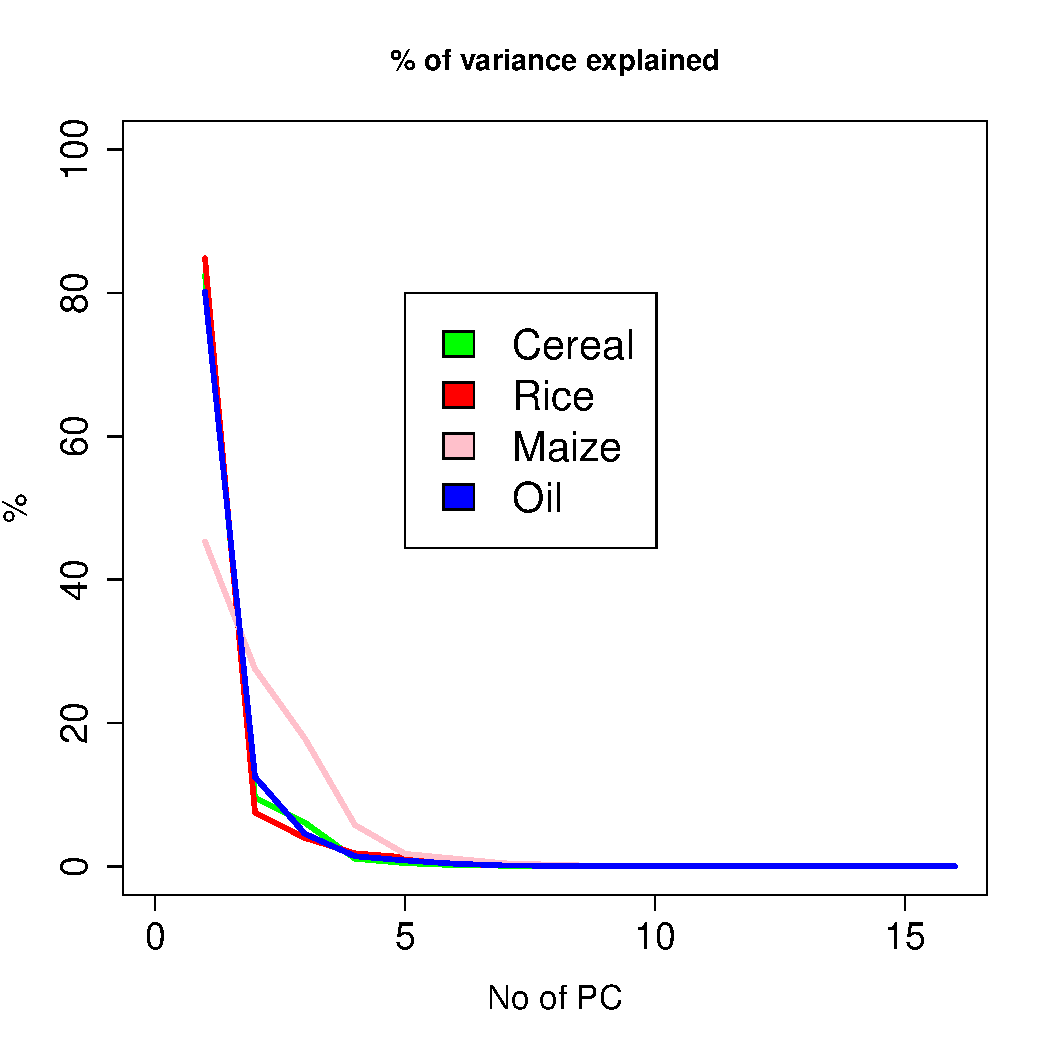
\includegraphics[width=1\textwidth]{GP/rain/PCA_rain2.pdf}
\caption[]{\% of the variance explained by each PC for the four rainfed crops. The plots correspond to crop-yield for management level of 5, RCP6 with CO$_2$ fertilization from UKMO-HADGEM1.}\label{pca}
\end{figure}

\begin{figure}[!ht]
\begin{subfigure}[h]{\textwidth}
\centering
\includegraphics[height=9cm,width=1.1\textwidth]{GP2/cereal1_rain.pdf}
\caption{LPJmL and emulator predictions including their 95\% C.I vs. UN country levels}
\label{myfigg9a1}
\end{subfigure}\\
\begin{subfigure}[h]{\textwidth}
\centering
\includegraphics[height=9cm,width=1.1\textwidth]{GP2/cereal2_rain.pdf}
\caption{Pair plot of emulator predictions vs. LPJmL values including their 95\% C.I}
\label{myfigg9a2}
\end{subfigure}
\caption{Cross-validation for rainfed cereal; LPJmL and emulator with its 95\% C.I for some countries levels.}\label{myfigg9a}
\end{figure}

Figure \ref{myfigg9a} is the GP emulation results for rainfed temperate cereal under RCP6, management level 5 and $8^{th}$ decadal change for UKMO-HADGEM1. Figure \ref{myfigg9a1} shows the performance of the 106 GP rainfed emulators for the cereal. Each GP corresponds to individual countries where the rainfed cereal crop is grown. 

The four countries with the largest change in yield are Tajikistan, Montenegro, Canada and Luxembourg see Table~ (\ref{country}) for a list of UN countries. Uruguay and Morocco are two countries with a large reduction in cereal yield. There is relatively little change in other countries. The observed values for LPJmL are well captured within the 95\% C.I of the emulator predictions. The emulator relatively well predicts Tajikistan with the largest change. Uruguay has the lowest change in yield and is under-predicted by emulator, with values $-1.21\pm 0.05$, -1.46 ton/Ha given respectively by emulator and LPJmL.

Figure \ref{myfigg9a2} is a bilinear plot between LPJmL and the emulator for 106 countries. The LPJmL values are arranged in ascending order from least to highest. The plot shows more clearly that the changes in yield for LPJmL are clustered together for most of the countries and are within 95\% C.I limit. The two end points correspond to Tajikistan and Uruguay, and uncertainties at either end are large as seen in the plot. The total percentage of variance explained by emulator for cereal is 92\%.

\begin{figure}[!ht]
\begin{subfigure}[h]{\textwidth}
\centering
\includegraphics[height=9cm,width=1.1\textwidth]{GP2/cereal1_irri.pdf}
\caption{LPJmL and emulator predictions including their 95\% C.I vs UN country levels.}
\label{myfig9a21}
\end{subfigure}\\
\begin{subfigure}[h]{\textwidth}
\centering
\includegraphics[height=9cm,width=1.1\textwidth]{GP2/cereal2_irri.pdf}
\caption{Pair plot of emulator predictions vs LPJmL values including their 95\% C.I}
\label{myfig9a22}
\end{subfigure}
\caption{Cross-validation for irrigated cereal yield; LPJmL and emulator with its 95\% C.I for some countries levels.}\label{myfig9a2}
\end{figure}


%The plot indicates a rise in yield for most countries except in South Africa and Denmark that have a large reduction in yield ($-0.12\pm 0.0085$, $-0.16\pm 0.085$ ton/H) respectively. In most countries, LPJmL values are within 95\% confidence level predicted by the emulator an indication of useful predictions. The Democratic Republic of Korea has large predictions than other countries $0.68\pm .11$ ton /Ha. Figure \ref{myfig9a22} is the bilinear plot between LPJmL and emulators. Again, most of the predicted values for countries are clustered together as we observed for rainfed. 
Figure \ref{myfig9a21} shows that the observed yield (LPJmL) and predicted (emulator) are mostly within 95\% C.I. 
Overall, we see that the cereal is well predicted for both rainfed and irrigated yields with majority of points lie within their uncertainty limits. Further test involves computing cross-validated root mean squared error (RMSE$_{CV}$) is given by equation \ref{gaga4b}. The values are 0.0082 and 0.0018 ton/Ha for rainfed and irrigated respectively. We can clearly see that predictions are much better (low RMSE$_{CV}$) for irrigated than for rainfed yields.

\begin{figure}[!ht] 
\includegraphics[width=1.1\textwidth]{GP2/sp_cereal2.pdf}
\caption[]{Cross-validation of the comparison between LPJmL and LPJmLem for rainfed and irrigated temperate cereals, plotted as mean decadal change in yield between (2085-2094) and (2005-2014) with their 95\% C.I. The plots correspond to crop-yield for management level of 5, RCP6 with CO$_2$ fertilization from UKMO-HADGEM1.}\label{Va}
\end{figure}
%%%%%%%%%%%%%%%%%%%%%%%%%%%%

\begin{figure}[!htb]%[!Ht]
\begin{subfigure}[b]{\textwidth}
\centering
\includegraphics[width=.69\textwidth]{GP2/per_cereal1.pdf}
\caption{Rainfed cereal}
\label{per1a}
\end{subfigure}\\
\begin{subfigure}[b]{\textwidth}
\centering
\includegraphics[width=.69\textwidth]{GP2/per_cereal2.pdf}
\caption{Irrigated cereal}
\label{per2a}
\end{subfigure}
\begin{subfigure}[b]{\textwidth}
\centering
\includegraphics[width=.69\textwidth]{GP2/per_rice1.pdf}
\caption{Rainfed rice}
\label{per3a}
\end{subfigure}
\begin{subfigure}[b]{\textwidth}
\centering
\includegraphics[width=.69\textwidth]{GP2/per_rice2.pdf}
\caption{Irrigated rice}
\label{per4a}
\end{subfigure}
\caption{Change in percentage yield by emulator with 95\% C.I. in comparison with LPJmL values for major producers of selected crops.}
\end{figure}

We show results for the major producing countries. In Figure~\ref{per1a}, emulator predictions are similar to LPJmL values except for India where the emulator under-predicts the change in yield. LPJmL produces about 17\% while emulator gives $13\pm 0.4\%$ for India. There is a substantial change in yield in the USA than for other major producers of cereal crop with both LPJmL and emulator estimate $\ge33\%$. 
For the irrigated cereal in Figure~\ref{per2a}, emulator predicts relatively well the change in yield for China, India and Russia. In each of this case, the LPJmL values are within the 95\% C.I band. Emulator under-predict the change in USA. There is a general increase in yield under climate change in these countries. The growth varies between 6-36\% across the country for both rainfed and irrigated crops. 

Consider Figures~\ref{per3a} and Figure~\ref{per4a}, China has a substantial change with a rise of 26\% in yield for rainfed and a growth of 30\% under irrigation. The emulator predicts $28\pm 0.18\%$ and $30\pm 2.2\%$ respectively. The results of other countries are relatively close except under rainfed in Bangladesh where the emulator under-predicts the yield. For irrigated rice, emulator under-predicts change in Indonesia and over-predicts the change for Bangladesh.
In Figure~\ref{per1b}, maize exhibits a slight increase in yield with the globally averaged yield change increasing
by 2\% in China and Brazil. In contrast, there is a relatively steady reduction in yield in USA and France as simulated by LPJmL. The emulator, on the other hand, seems to be badly behaved as the values are poorly predicted by the emulator. For instance, while the LPJmL produces a growth of 2.5\% in Brazil, emulator projects a reduction of $1.2\pm0.12\%$. In France, LPJmL gives a decline of 1.5\% emulator predicts a rise of $4\pm1\%$.

Emulator predictions under irrigation in Figure~\ref{per2b} are much better than for rainfed maize. LPJmL values are within 95\% confidence band. There is a slight increment in yield of less than 3\% in China and USA while France has a considerable large growth of 20\%. However, there is a decline in maize yield in Brazil. Figure~\ref{per3b} shows a large increment of more than 60\% in Argentina oil and Figure \ref{per4b} indicates a modest increase in oil yield in Brazil. The emulator predicts better result in comparison with LPJmL values.

Overall, there is an increase in yield for most of the countries as expected because of the beneficial effect of CO$_2$ fertilization included in this simulation. However, maize shows a reduction in yield in USA, France and Brazil.


\begin{figure}[!htb]
\begin{subfigure}[b]{\textwidth}
\centering
\includegraphics[width=.69\textwidth]{GP2/per_maize1.pdf}
\caption{Rainfed maize}
\label{per1b}
\end{subfigure}\\
\begin{subfigure}[b]{\textwidth}
\centering
\includegraphics[width=.69\textwidth]{GP2/per_maize2.pdf}
\caption{Irrigated maize}
\label{per2b}
\end{subfigure}
\begin{subfigure}[b]{\textwidth}
\centering
\includegraphics[width=.69\textwidth]{GP2/per_oil1.pdf}
\caption{Rainfed oil}
\label{per3b}
\end{subfigure}
\begin{subfigure}[b]{\textwidth}
\centering
\includegraphics[width=.69\textwidth]{GP2/per_oil2.pdf}
\caption{Irrigated oil}
\label{per4b}
\end{subfigure}
\caption{Change in percentage yield by emulator with 95\% C.I. in comparison with LPJmL values for major producers of selected crops.}
\end{figure}

%%%%%%%%%%%%%%%%%%%%%%%%%%%%%%
%Now, let's look at the spatial map of the rainfed cereal more clearly in Figure~\ref{Va} (top)
We now consider the spatial map of rainfed cereal in Figure~\ref{Va} (top) in more detail.  The white coloration in this map represents regions that are not currently growing cereal crop. Most of the countries are reasonably well-predicted. The Russia Republic and Canada are under-predicted by the emulator. For instance, while the LPJmL simulates increase in yield of 0.52 and 0.90 ton/Ha for the Russia Federation and Canada, emulator predicts growth of $0.49\pm0.01 $ and $0.61\pm0.09$ ton/Ha respectively. Predicted values by the emulator are higher than for the LPJmL values for Mongolia, Tajikistan and South Africa. For instance, while LPJmL gives increase in yield of 0.20 ton/Ha emulator produces $0.38\pm 0.003$ ton/Ha for South Africa.

Emulators predict increases in yield, as does LPJmL for most of the countries under this scenario. This increase is expected because of beneficial CO$_2$ effect. There are significant yield changes for Europe, China, USA, Russia, and these countries have in common a well-managed land system. In addition, increasing in warming conditions, as projected under climate change will give rise to prolonged growing season in these regions that will cause an increase in yield \citep{q88,q85,q91}. In particular, \cite{q90} associated significant increases in food production in China to technological advancement and changing in agronomic practices in that country.

Yield changes are significantly higher for high latitude and middle than for low latitudes in agreement with some literatures \citet{n11,42b,n12}. %and especially in UK and northeast China \citep{q70}. 
Climate change will cause low latitude to experience a greater degree of heat and water stress which will cause a decline in yield even in the presence of the CO$_2$ fertilization effect. For instance, in Australia there is a fairly little change in yield that could probably due to a large variability in precipitation, extended droughts and a greater incidence of extreme weather events in this region which could disrupt agricultural production. In addition, Australia and New Zealand exhibit a wide diversity of climates with a significant constraint on water resources as described in \citep{q85}. Algeria, Ireland, Morocco and Uruguay also have a substantial reduction in yield. Uncertainty levels are low and vary from one country to another because each country is modelled by an independent Gaussian process regression.


Under irrigation, Figure~\ref{Va} (bottom) yield change are relatively lower in USA, China and Russia compare to rainfed system unlike Canada that has a larger increase yield than for rainfed. Reduction in crop yield is large in Argentina, Yemen, South Africa and Ethiopia. Increase in yield changes is substantial for Canada, Armenia and Spain. Similar to rainfed cereal, lower yield changes are associated with medium and low latitude countries than for high latitude countries. 
Crossvalidation maps for other crops are shown in Appendix 5.

We summarise the results of the emulator in Table \ref{GPtab2} for all management levels, RCP and time point with CO$_2$ fertilization for UKMO-HADGEM1. We also compare the performance of the GP emulator with the WLS techniques. In this case, we use the same procedure set out in this paper but instead of performing GP regression we used the WLS approach. Proportion of variances explained is shown below.
Table \ref{GPtab2} indicate that GP regression is slightly better than the WLS method for all the cases except for rainfed oil. Irrigated cereal and maize results are much better under GP models than for WLS approach. However, the two techniques produce relatively similar results for irrigated rice and oil. GP emulator explains between 70-94\% variance while WLS ranges from 63-93\% for both rainfed and irrigated crops. 

Consider cross-validation for four additional GCMs in Table~\ref{GPtab3}. We see that CCSR-MIROCMED results are much better than for other GCMs as expected because a very similar GCM, CCSR-MIROC32HI, was part of the training data. Results from GP models are much better than WLS technique among all GCMs except for rice under IPSL-CM4 where the result is slightly better than for GP models.

\begin{table*}[!ht] 
\caption{Table of cross-validated proportion of variance $\rho$ showing the overall performance of the GP emulators, and in comparison with WLS method, for rainfed and irrigated crops, with all management levels, RCPs, and time slices, but with CO$_2$ fertilization only. The list of countries are shown in Table \ref{country}.}
\label{GPtab2}
\begin{tabular}{|c|cc|cc|ccc|}
\hline
$\rho$ &Number of countries& & GP&&WLS&& \\
\hline
crops&rainfed&irrigated& rainfed&irrigated&rainfed&irrigated& \\
\hline
cereal&106&83 & 0.89&0.94&0.81&0.87&\\ 
\hline
rice& 79 & 95&0.82&0.92&0.77&0.93&\\ 
\hline
maize &141 &100 &0.70&0.80&0.63&0.76&\\ 
\hline
oil$_{max}$ &139 &64 &0.89&0.88&0.91&0.88&\\ 
\hline
\end{tabular}
\end{table*}


\begin{table*}%[!ht]
%\centering
\small{
\caption{Comparison of GP with WLS methods for four GCMs, with CO$_2$ fertilization, management level 5, RCPs 4.5 and 8.5, and all time slices for rainfed crops. The values are the proportion of variance $\rho$ explained.}
\label{GPtab3}
\begin{tabular}{lccccccccccc}
\hline
Crop&\multicolumn{2}{c}{CCSR-}&&\multicolumn{2}{c}{GISS-}&
&\multicolumn{2}{c}{GISS-}&&\multicolumn{2}{c}{IPSL-}\\
&\multicolumn{2}{c}{MIROCMED}&&\multicolumn{2}{c}{MODELER}&
&\multicolumn{2}{c}{MODELEH}&&\multicolumn{2}{c}{CM4} \\
\cline{2-3} \cline{5-6} \cline{8-9} \cline{11-12}
&GP& WLS&& GP&WLS&&GP&WLS&&GP&WLS \\
\hline
\vspace{.2in}
Cereal&0.87& 0.81&& 0.71&0.66&&0.78&0.72&&0.75&0.72\\
\vspace{.2in}
Rice& 0.83 & 0.81&&0.71&0.67&&0.83&0.67&&0.71&0.72\\
\vspace{.2in}
Maize & 0.92& 0.86&&0.69&0.67&&0.76&0.68&&0.87&0.80\\
\vspace{.2in}
Oil$^1$ &0.89 & 0.83&&0.84&0.78&&0.83&0.74&&0.83&0.77\\
\hline \vspace{-.1in}
\end{tabular}\\
{\footnotesize $^1$ Oil=yield$_{max}$[soybean, rapeseed, sunflower].\\} }
\end{table*}

\begin{figure}[!Ht]
\begin{subfigure}[h]{\textwidth}
\centering
\includegraphics[height=.35\textwidth,width=.9\textwidth]{GP2/percent_rain.pdf}
\caption{Rainfed crops}
\label{global1}
\end{subfigure}\\
\begin{subfigure}[h]{\textwidth}
\centering
\includegraphics[height=.35\textwidth,width=.9\textwidth]{GP2/percent_irri.pdf}
\caption{Irrigated crops}
\label{global2}
\end{subfigure}
\caption{Global percentage change in yield by emulator with its 95\% C.I. in comparison with LPJmL values for a period (2085-2094) relative to ($2005-2014$) with their 95\% C.I. The plots correspond to crop-yield for management level of 5, RCP6 with CO$_2$ fertilization from UKMO-HADGEM1.}
\end{figure}

Figures \ref{global1} average global changes in yield predicted by emulator in all countries and compare to LPJmL values.
Emulator predicts global average change in yield for cereal and rice relatively well with 14\% and 13\% respectively with LPJmL values within 95\% C.I. Maize and oil crops are under-predicted by the emulator. Predicted maize values from the emulator are much lower to the LPJmL values. LPJmL simulates a small increase of 1.9\% for maize; emulator predicts a reduction of -0.25\%. Figure \ref{global2} for irrigated crops indicated that the oil is under-predicted by the emulator, while emulator predictions produce for cereal, rice and maize are relatively similar to LPJmL values. Uncertainty interval is much higher in oil than for other crops. Comparing the two plots irrigated rice and maize global percentage changes in yield are higher than for rainfed rice and maize. In contrast, irrigated cereal and oil percentage changes are comparatively less than for rainfed crops.


\section{Discussion}
The reason for applying the GP on residual from model results instead of the simulation data. Our simulation data for both crops and climate are high-dimensional gridded global data that cannot be modelled directly by GP. Several approximation techniques have been developed to handle multi-dimensional data. For instance, a low-rank approximation of the Gram matrix was described in \cite{q10,q11}. The use of subsets of regressors and subsets of data to reduce the computational burden of the GP inversion for a large data matrix was investigated by \cite{q12,q13,q14}. The following studies used Bayesian techniques for emulating high-dimensional data \cite{q28,q29,q22,q23,qq}. In particular, \cite{r3,qq62} used Bayesian methods for predicting crop yields. A good emulator must be as fast as possible to allow for relatively quick evaluation of many scenarios which are not feasible with these techniques. Therefore, the Bayesian procedures used in the studies mentioned above cannot be directly applied to handle large dimensional and high-resolution crop data in this study. 

Secondly, climate varies considerably from one spatial scale to another. This variability is determined largely by atmospheric circulation and its interactions with large-scale ocean currents. Regional or local climate is much more variable than global climate because climate on a large spatial scale is less influenced by internal dynamics of the continental or global climate. Therefore, even if we decide to use a PC decomposition or aggregation of the crop yields data (to reduce the dimension). We may not be able to apply that data reduction strategy to climate input parameters as they vary from one location to another. 
The decomposition of the data is non-trivial as climate may vary a lot within a  country so that the average climate across a country may be a poor approximation to the local climates within the country. In addition, LPJmL data is a non-linear response so large scale average climate may be an inappropriate input to our problem.

Thirdly, the LPJmL data that we are using are monthly data and they have been averaged to decadal level. We have already lost some information due to decadal averaging because the LPJmL model itself works on a daily time step. We do not want to lose further vital information from the data by further averaging or by applying principal components to reduce the dimension of our data. Applying PCA  to reduce dimension of LPJmL will cause significant loss of information at early stage of the modelling. The resulting PC components will ignore information about the climate input variables thereby giving rise to PC components that might be difficult to explain by the original input variables. In order to proceed, we decided to emulate the high-dimensional data at a high spatial resolution using stepwise regression. We project the predictions and residuals obtained from stepwise regression results to a lower dimension by aggregating spatially to country levels. Then apply a GP regression for residuals interpolation from the new projected axes.

Another way to resolve our problem is to treat each spatial point as a GP and then emulate each grid cell individually a technique implemented in \cite{q62} and \cite{q64}. However, this option is intractable since we have 59199 grid points meaning that about 236,796 emulators have to be constructed and validated for the four crops we are emulating.

\section{Conclusion}
In this paper, we have demonstrated a means of making inference about the parameters of the emulator using a GP regression that is based upon Bayesian principle. We have presented a simple statistical method for emulating the underlying physical dynamics of response of potential crop yield to change in climate. We use combinations of stepwise regression, PCA and GP methods to emulate major crop-yield as a linear function of seasonal climate variables and other relevant variables. Aggregated country average of actual yield change is calculated by combining yields simulated by LPJmL for both rainfed and irrigated. We consider eight time-slices averaged over ten years, baseline corresponding to the average (2005-2014). 

In modelling the residual $\bZ$, we reduced the complexity of the computation by aggregating the stepwise regression residuals from a fine to a more coarse resolution on a country level. We assume that the aggregation will reduce the complexity and structure of the global trend component of the emulator. We have already seen from the residual plots that some variations have not been accounted for by the stepwise regression model.

We demonstrated in \cite{qwole} that the stepwise regression approach captures some proportion of the global variation in our data. The residual analysis is performed to capture the remaining spatial local variation left unexplained in stage 1. In Bayesian framework, we assumed that our unexplained residual from stage1 is a GP. Under GP regression, we specified both the prior mean and covariance functions and estimated the hyperparameters of these functions by integrating out the nuisance parameters using the Bayes rule. 

It is important to reduce the dimensionality of data for tractable application of GP modelling. We derived the input matrix $\tbU$ from the stage 1 predictions, this matrix was then used as explanatory variables for GP regression. We first obtained the residual on a lower axis by aggregating to a country level. We fitted an independent GP in parallel to each column of $\bf Z$. These emulators can predict the change in global crop yield as a function of climate from any GCM/RCP combination and for different management level options and CO$_2$ fertilization level. We provided some spatial plots to compare the performance of the emulators with the LPJmL.

Overall, cereal is more predictable in South America, Africa and China than other part of the world. Similarly, rainfed rice is more predictable in North America, China and India but is more difficult to predict in Australia. Maize and oil are generally much predictable in most regions except in Canada and Mongolia. Uncertainty levels are also relatively low for all the four crops. There are some isolated large confidence bands in some countries which could be attributed to a large variability in the training data for these countries. The large uncertainty can be traced to inter-scenario variabilities across RCP and GCM.
 
\begin{table}[ht]
\caption{List of UN countries used for this analysis}\label{country}
\scriptsize
\begin{tabular}{r|r|r|r|r|r|}
\hline
Index&Country &Index&Country&Index&Country\\ 
\hline
1 &Ocean & 63 & French Polynesia & 125& New Zealand \\ 
2 & Afghanistan & 64 & French Southern Territories & 126& Nicaragua \\ 
3 & Albania & 65 & Djibouti & 127& Niger \\ 
4 & Antarctica & 66 & Gabon & 128 &Nigeria \\
5 & Algeria & 67 & Georgia & 129& Norway \\ 
6 & Angola & 68 & Gambia & 130& Pakistan \\ 
7 & Azerbaijan &69 & State of Palestine & 131& Panama \\ 
8 & Argentina & 70 & Germany & 132& Papua New Guinea \\ 
9 & Australia & 71 & Ghana & 133& Paraguay \\ 
10 & Austria & 72 & Kiribati & 134& Peru \\ 
11 & Bahamas & 73 & Greece & 135& Philippines \\ 
12 & Bangladesh & 74 & Greenland & 136 &Poland \\ 
13 & Armenia & 75 & Guatemala & 137& Portugal \\ 
14 & Belgium & 76 & Guinea & 138 & Guinea-Bissau \\ 
15 & Bhutan & 77 & Guyana & 139& Timor-Leste \\ 
16 & Bolivia & 78 & Haiti & 140& Puerto Rico \\ 
17 & Bosnia and Herzegovina & 79 & Honduras & 141& Qatar \\ 
18 & Botswana & 80 & Hungary & 142& Romania \\ 
19 & Brazil & 81 & Iceland & 143& Russian Federation \\ 
20 & Belize & 82 & India & 144& Rwanda \\ 
21 & Solomon Islands & 83 & Indonesia & 145 & Saint Vincent and Grenadines \\ 
22 & Brunei Darussalam & 84 & Iran & 146 & Saudi Arabia \\ 
23 & Bulgaria & 85 & Iraq & 147 & Senegal \\ 
24 & Myanmar & 86 & Ireland & 148 & Serbia \\ 
25 & Burundi & 87 & Israel & 149 & Sierra Leone \\ 
26 & Belarus & 88 & Italy & 150 & Slovakia \\ 
27 & Cambodia & 89 & Cote d'Ivoire & 151 & Viet Nam \\ 
28 & Cameroon & 90 & Jamaica & 152 & Slovenia \\ 
29 & Canada & 91 & Japan & 153 & Somalia \\ 
30 & Cape Verde & 92 & Kazakhstan & 154 & South Africa \\ 
31 & Cayman Islands & 93 & Jordan & 155 & Zimbabwe \\ 
32 & Central African Republic & 94 & Kenya & 156 & Spain \\ 
33 & Sri Lanka & 95 & Democratic Republic of Korea & 157 & South Sudan \\ 
34 & Chad & 96 & Republic of Korea & 158 & Sudan \\ 
35 & Chile & 97 & Kuwait & 159 & Suriname \\ 
36 & China & 98 & Kyrgyzstan & 160 & Swaziland \\ 
37 & Taiwan & 99 & Lao Republic & 161 & Sweden \\ 
38 & Colombia & 100 & Lebanon & 162 & Switzerland \\ 
39 & Comoros & 101 & Lesotho & 163 & Syrian Arab Republic \\ 
40 & Congo & 102 & Latvia & 164 & Tajikistan \\ 
41 & D.R Congo & 103 & Liberia & 165 & Thailand \\ 
42 & Costa Rica & 104 & Libya & 166 & Togo \\ 
43 & Croatia & 105 & Lithuania & 167 & Trinidad and Tobago \\ 
44 & Cuba & 106 & Luxembourg & 168 & United Arab Emirates \\ 
45 & Cyprus & 107 & Madagascar & 169 & Tunisia \\ 
46 & Czech Republic & 108 & Malawi & 170 & Turkey \\ 
47 & Benin & 109 & Malaysia & 171 & Turkmenistan \\ 
48 & Denmark & 110 & Mali & 172 & Uganda \\ 
49 & Dominican Republic & 111 & Mauritania & 173 & Ukraine \\ 
50 & Ecuador & 112 & Mauritius & 174 & The former Yugoslav \\ 
51 & El Salvador & 113 & Mexico & 175 & Egypt \\ 
52 & Equatorial Guinea & 114 & Mongolia & 176 & United Kingdom \\ 
53 & Ethiopia & 115 & Republic of Moldova & 177 & United Republic of Tanzania \\ 
54 & Eritrea & 116 & Montenegro & 178 & United States of America \\ 
55 & Estonia & 117 & Morocco & 179 & United States Virgin Islands \\ 
56 & Faeroe Islands & 118 & Mozambique & 180 & Burkina Faso \\ 
57 & Falkland Islands (Malvinas) & 119 & Oman & 181 & Uruguay \\ 
58 & South Georgia and South SS & 120 & Namibia & 182 & Uzbekistan \\ 
59 & Fiji & 121 & Nepal & 183 & Venezuela \\ 
60 & Finland & 122 & Netherlands & 184 & Samoa \\ 
61 & Aland Islands & 123 & New Caledonia & 185 & Yemen \\ 
62 & France & 124 & Vanuatu & 186 & Zambia \\ 
\hline 
\end{tabular}
\end{table}



%\begin{acknowledgements}
%If you'd like to thank anyone, place your comments here
%and remove the percent signs.
%\end{acknowledgements}

% BibTeX users please use one of
%\bibliographystyle{spbasic}      % basic style, author-year citations
%\bibliographystyle{spmpsci}      % mathematics and physical sciences
%\bibliographystyle{spphys}       % APS-like style for physics
%\bibliography{}   % name your BibTeX data base

% Non-BibTeX users please use
%\begin{thebibliography}{}


%\end{thebibliography}
\newpage
\section*{Appendix 1: GP derivation}
Let $\mathbf{z}=[(z_i,f(u_i)|i=1,\ldots,n)]^T$ be some simulation data and given some prior distribution for hyperparameters. Then 
\begin{equation}\tag{A.1}\label{gpr2}
P(\boldsymbol\beta,\sigma^2|\mathbf{z})=\frac{P(\mathbf{z}|\boldsymbol\beta,\sigma^2) P(\boldsymbol\beta,\sigma^2)} {P(\mathbf{z})}\propto P(\mathbf{z}|\boldsymbol\beta,\sigma^2) P(\boldsymbol\beta,\sigma^2) 
\end{equation}
where $P(\boldsymbol\beta,\sigma^2|\mathbf{z})$ is the parameter posterior distribution, $P(\mathbf{z}|\boldsymbol\beta,\sigma^2)$ is the likelihood, $P(\boldsymbol\beta,\sigma^2)$ the prior distribution for hyperparameters. The marginal likelihood or normalising factor $P(\mathbf{z})$ can also be expressed as
\begin{equation}\tag{A.2}\label{gpr2c}
P(\mathbf{z})=\int P(\mathbf{z}|\boldsymbol\beta,\sigma^2) P(\boldsymbol\beta,\sigma^2)~ d\boldsymbol\beta ~d\sigma^2
\end{equation}
under a full Bayesian framework, the posterior distribution in equation \ref{gpr2} and the marginal distribution in equation \ref{gpr2c} are often difficult to compute for any arbitrary prior distribution, they may not exist in closed form. Conjugate or non-informative priors can be used to overcome this non-analyticity. A conjugate distribution arises when both the posterior and prior distributions come from the same family. %A prior \rho(\boldsymbol\beta,\sigma^{2}) is conjugate to this likelihood function if it has the same functional form with respect to \boldsymbol\beta and \sigma.
Suppose, we want to make prediction at a new design point $u^{new}$ given some training data $\bf z$, then the joint distribution of the observed values $\bf z$ and test point $z^{new}$ under a given prior can be obtained. $\bf z$ is 
\begin{equation}\tag{A.3}\label{gpr0} 
\bf z\sim N(\bf H\boldsymbol \beta,\sigma^2\bf C)
\end{equation}
and $z^{new}=f(u^{new})$ have a joint multivariate Gaussian distribution using multivariate identity. Then we have
\begin{equation}\tag{A.4}\label{gpr2d}
z^{new}|\bf z, \boldsymbol\beta,\sigma^2 \sim N[m^{\star}(.),\sigma^2C^{\star}(.,.)].
\end{equation}
such that
$$m^{\star}(\mathbf{u})=h^{T}(\mathbf{u})\boldsymbol\beta+\bf cC^{-1}[z-H(u)\boldsymbol\beta]$$
$$ C^{\star}(\mathbf{u,u'})=c(\mathbf{u,u'})-\bf c(\mathbf{u})^T C^{-1}c(\mathbf{u'}),$$ 
%where $\bf H^T=[h(u_1,\ldots,h(u_n)]$ and $\mathbf{c(u)}^T=[c(u,u_1),\ldots,c(u,u_n)]$ is the correlation between the training and test points. The correlation matrix of the input (training) design matrix is given by
%\begin{equation}
%\mathbf{C}=
%\begin{pmatrix}
%1 &c(u_1,u_2) & \ldots & c(u_1,u_n) \\
%c(u_2,u_1) & 1 & \ddots&\vdots \\
%\vdots & \ddots &\ddots &\vdots\\
%c(u_n,u_1) & \ldots & \ldots& 1
%\end{pmatrix}
%\end{equation}

In order to make predictions, we integrate over the posterior distribution (i.e. the expectation of the posterior density). Therefore, the posterior predictive density is given by
\begin{equation}\tag{A.5}\label{gpr3}
P(z^{new}|\mathbf{z})=\int_{d\boldsymbol\beta}\int_{d\sigma^2} P(z^{new}|\boldsymbol\beta,\sigma^2) P(\boldsymbol\beta,\sigma^2|\mathbf{z})~ d\boldsymbol\beta ~d\sigma^2.
\end{equation}
As mentioned, it can be difficult to obtain the $P(z^{new}|\mathbf{z})$ analytically. %in order to continue, approximation technique like maximum likelihood function can be used instead for the integration. 
The joint prior distribution $P(\boldsymbol\beta,\sigma^2|\mathbf{z})$ in equation \ref{gpr3} can be further re-expressed below using the probability product identity
\begin{equation*}
P(\boldsymbol\beta,\sigma^2|\mathbf{z})=P(\boldsymbol\beta|\sigma^2,\mathbf{z}) P(\sigma^2|\mathbf{z}).
\end{equation*}
Let the prior distribution on the regression parameter $\boldsymbol\beta$ and $\sigma^2$ be given by a weak prior such that
\begin{equation}\tag{A.6}\label{gpr3b}
P(\boldsymbol\beta, \sigma^2) \propto \frac{1}{\sigma^2}
\end{equation}
Substituting equations (\ref{gpr0} and \ref{gpr3b}) to the posterior distribution in equation \ref{gpr2} and with little algebraic manipulation we can infer that $P(\boldsymbol\beta|\sigma^2,\mathbf{z})\sim N(\boldsymbol{\hat\beta},\sigma^2 (HC^{-1}H)^{-1})$ and $\sigma^{2}|\bf z$ has an inverse-gamma distribution where $P(\sigma^{2}|\mathbf{z})=\int P(\sigma^2, \boldsymbol\beta|\mathbf{z})d\boldsymbol{\beta}\sim (n-p-2)\hat \sigma^2\chi_{(n-p)}^{-2}$.
Let $\boldsymbol{\hat\beta}$ and $\hat \sigma^2$ be the MLE values of $\boldsymbol{\beta}$ and $\sigma^2$, to be discussed shortly in Appendix 2.
Therefore, the estimates of $\boldsymbol\beta$ and $\sigma^2$ are obtained by integrating over all hyperparameters values weighted by their posterior.
Therefore, equation \ref{gpr3} can be expressed as
\begin{equation*}\label{gpr4}
P(z^{new}|\mathbf{z})=\int_{d\boldsymbol\beta}\int_{d\sigma^2} P(z^{new}|\boldsymbol\beta,\sigma^2)P(\boldsymbol\beta|\sigma^2,\mathbf{z}) P(\sigma^2|\mathbf{z}) ~ d\boldsymbol\beta ~d\sigma^2,
\end{equation*}
$$\approx \int_{d\boldsymbol\beta}\int_{d\sigma^2} P(z^{new}|\boldsymbol\beta,\sigma^2)P(\boldsymbol\beta|\sigma^2,\mathbf{z}) (n-p-2)\hat \sigma^2\chi_{(n-p)}^{-2} ~ d\boldsymbol\beta ~d\sigma^2$$
%$$=\int_{d\boldsymbol\beta} P(z^{new}|\boldsymbol\beta,\hat\sigma^2)P(\boldsymbol\beta|\hat\sigma^2,\mathbf{z}) ~ d\boldsymbol\beta. $$
$$=(n-p-2)\hat \sigma^2\chi_{(n-p)}^{-2} \int_{d\boldsymbol\beta} P(z^{new}|\boldsymbol\beta,\hat \sigma^2)P(\boldsymbol\beta|\hat \sigma^2,\mathbf{z})d\boldsymbol\beta.$$
The values of the integrand can be evaluated noting that the first term in the integral follows from equation (\ref{gpr2d}), and also recognise that $P(\boldsymbol\beta|\hat \sigma^2,\mathbf{z})\sim N(\boldsymbol{\hat\beta},\hat\sigma^2 (HC^{-1}H)^{-1})$ (product of two Gaussian distribution). Therefore,
\begin{equation}\tag{A.7}\label{gpr5}
P(z^{new}|\mathbf{z})=(n-p-2)\hat \sigma^2\chi_{(n-p)}^{-2}\times N[m^{\bullet}(.),\sigma^2C^{\bullet}(.,.)].
\end{equation}
where
\begin{equation}\tag{A.8}\label{olu1}
m^{\bullet}(\mathbf{u})=h^{T}(\mathbf{u})\boldsymbol{\hat\beta}+\bf cC^{-1}[z-H(u)\boldsymbol{\hat\beta}]
\end{equation}
\begin{equation}\tag{A.9}\label{olu2}
C^{\bullet}(\mathbf{u,u'})=C^{\star}(\mathbf{u,u'})\bf+ \Big[(h(u)^T c(u)C^{-1}H)(H^TC^{-1}H)^{-1}(h(u)^T c(u)C^{-1}H)^T\Big],
\end{equation}
\begin{equation*}\label{gpr5}
P(z^{new}|\mathbf{z})=T_{(n-p)}\Big(m^{\bullet}(\mathbf{u}), \frac{(n-p)C^{\bullet}(\mathbf{u,u'})}{(n-p-2)}\Big)
\end{equation*}
where $T_{(n-p)}$ is a student $t$ distribution with $(n-p)$ degree of freedom \citep{q35,qq64,q9}.

\section*{Appendix 2: Estimation of prior hyperparameters}\label{hyper}
Noting that under GP regression, the prior distribution for the data is also a Gaussian distribution.
Let the log-likelihood of the parameters be given as
\begin{equation}\tag{A.10}\label{like}
L(\boldsymbol \beta, \sigma^2, \boldsymbol{\alpha})=-\frac{1}{2}\Big[n~log(\sigma^2)+log(det(\bf C))+(z-H\boldsymbol \beta)^T \bf C^{-1}(z-H\boldsymbol \beta)/\sigma^2\Big]
\end{equation}
where $\boldsymbol{\alpha}=[\alpha_1, \ldots, \alpha_n]$ is a vector of correlation lengths and $det(\bf C)$ is the determinant of correlation matrix $\bf C$. Maximizing this function with respect to $\boldsymbol \beta$ will give the MLE of $\boldsymbol \beta$ as (also equal to its generalized least squares estimate)
\begin{equation}\tag{A.11}
\hat{\boldsymbol \beta}=(\mathbf{H^TC^{-1}H)}^{-1}\bf H^TC^{-1}z
\end{equation}
and for $\sigma^2$ as 
\begin{equation}\tag{A.12}
\widehat{\sigma^2}=\frac{1}{n}\Big[\mathbf{(z-H\hat{\boldsymbol \beta})}^T\bf C^{-1}(\bf z-H\hat{\boldsymbol \beta})\Big]
\end{equation}
In order to compute the MLE of $\boldsymbol{\alpha}$, the estimates of $\hat{\boldsymbol \beta}$ and $\widehat{\sigma^2}$ are substituted in equation (\ref{like}) and maximized over $\boldsymbol \beta$ and $\sigma^2$ to obtain
\begin{equation}\tag{A.13}
L(\hat{\boldsymbol \beta},\widehat{\sigma^2},\boldsymbol{\alpha})=-\frac{1}{2}\Big[n~log(\widehat{\sigma^2})(\boldsymbol{\alpha})+log(det(\bf C(\boldsymbol{\alpha})))+\textnormal n\Big],
\end{equation}
which is a function of $\boldsymbol{\alpha}$ that can be computed using a derivative-free numerical optimisation like Nelder-Mead method see further details in \citep{70,q10}.
Posterior distribution is obtained as $P(\mathbf{z}|\widehat{\boldsymbol\beta},\hat\sigma^2,\hat\alpha)\sim N[m^{\bullet}(u),\sigma^2C^{\bullet}(u,u')]$, with posterior mean and covariance functions given as equations (\ref{olu1} and \ref{olu2}) respectively.
%\begin{equation}
%m^{\bullet}(\mathbf{u})=h^{T}(\mathbf{u})\boldsymbol{\hat\beta}+\bf c(\mathbf{u})C^{-1}\Big[z-H(u)\boldsymbol{\hat\beta}\Big]
%\end{equation}
%and posterior covariance
%\begin{equation}
%C^{\bullet}(\mathbf{u,u'})=C^{\star}(\mathbf{u,u'})\bf+ \Big[(h(u)^T c(\mathbf{u})C^{-1}H)(H^TC^{-1}H)^{-1}(h(u)^T c(\mathbf{u})C^{-1}H)^T\Big],
%\end{equation} 
%Advantage of GP method is  that the prediction is probabilistic by providing confidence interval as a measure of uncertainty. GP is a robust method because it allows for different correlation and linear regression functions. Additional information in the form of a prior distribution improves the prediction. However, it efficiency reduces for high-dimensional data (scale poorly).


\section*{Appendix 3: Spatial aggregation procedure}\label{spap}
 In order to apply the GP regression for residual interpolation, we reduce the resolution of the residuals data from half degree to a country level by aggregating the residual matrix $\bE^{\rm T}$. For the evaluation of GP regression of residual, country-level residual values are computed by multiplying the residual at each grid cell by the crop growing area for each cell and separately for rainfed and irrigated crops. We calculated the area-weighted sum for each country to determine the total residual for that country, and finally dividing this total residual by the total (country) area. %Grid cells at which LPJmL was not simulated for each decade are discarded from this analysis. 

Therefore, for any $i^{th}$ residual scenario, 
\begin{equation}\label{agg1}
\mathbf{Z}_{[i,n]}=\frac{\sum \limits_{j=1}^{m} \bE^{\rm T}_{[i,j]}\times \mathbf{A}_j }{\sum \limits_{j=1}^{m} \mathbf{A}_{j}}
\end{equation} 
where $m$ is the number of grid cells that fall into country $n$, $\bE$ is the residual as defined earlier and $\mathbf{A}_j$ is the crop growing area for the $j^{th}$ grid cell and $i=(1,\ldots,16)$, $j=(1,\ldots,N)$. %This analysis is performed with $rworldmap$ package in $R$. The package documents the aggregation of global half degree gridded data to a country level for further detail see \cite{qq63}. 

\section*{Appendix 4: Model performance}
We compute the squared differences between the actual LPJmL values $y$ and $\bar y$ and also compute the squared differences between the LPJmL values and the emulator predictions. The proportion of the variance in the LPJmL values that is explained by the emulator is
%\begin{equation}
\begin{align}\label{gaga4}
\rho=1-\left[\frac{\sum\limits_{i=1}^{4}\sum\limits_{j=1}^{2}
\sum\limits_{k=1}^7\sum\limits_{t=1}^8\sum\limits_{n=1}^N
(y_{ijktn}-\tby_{ijktn}^{\star})^2}
{\sum\limits_{i=1}^{4}\sum\limits_{j=1}^{2}
\sum\limits_{k=1}^7\sum\limits_{t=1}^8\sum\limits_{n=1}^N
(y_{ijktn}-\bar y)^2}\right]
\end{align}
and the overall cross-validation root mean squared error (RMSE$_{CV}$) is
\begin{equation}\label{gaga4b}
\mbox{RMSE}_{CV}= \left(
\sum\limits_{i=1}^{4}\sum\limits_{j=1}^{2}
\sum\limits_{k=1}^7\sum\limits_{t=1}^8\sum\limits_{n=1}^N
\frac{(y_{ijktn}-\tby_{ijktn}^{\star})^2}{(4\times2\times7\times8\times N)} \right)^{1/2}.
\end{equation}


\begin{table*}[!ht]
\footnotesize
%\scriptsize
\begin{center}
\caption{The emulator's input variables for stepwise regression.}\label{tt1}
%\begin{tabular}{lcl}
\begin{tabular}{|c|cc|}
\hline
Variables& Full names&\\
\hline
&2001-2100  &\\
\hline
scld/weld/spcld/acld & Change in mean cloud cover in summer/winter/spring/autumn&\\
spre/wpre/sppre/apre & Change in mean precipitation in summer/winter/spring/autumn&\\
stmp/wtmp/sptmp/atmp & Change in mean temperature in summer/winter/spring/autumn &\\
swet/wwet/spwet/awet & Change in mean wet day frequency in summer/winter/spring/autumn &\\
iscld/iweld/ispcld/iacld & Initial (baseline) mean cloud cover in summer/winter/spring/autumn &\\
ispre/iwpre/isppre/iapre & Initial mean precipitation in summer/winter/spring/autumn &\\
istmp/iwtmp/isptmp/iatmp & Initial mean temperature in summer/winter/spring/autumn &\\
iswet/iwwet/ispwet/iawet & Initial wet day frequency in summer/winter/spring/autumn &\\
CO$_2$ and CCO$_2$ & Initial (baseline) mean CO$_2$ and change in mean CO$_2$ &\\
soil, lat and LAI & Soil and latitude parameters, and maximum leaf area index &\\
\hline
\end{tabular}
\end{center}
In the northern hemisphere, {\em summer} = \{June July August\}, {\em winter} = \{December January February\}, {\em spring} = \{March April May\} and {\em autumn} = \{September October November\}; obvious changes are made for the southern hemisphere.
\end{table*}

\section*{Appendix 5: Other results}
Next, we extend our cross-validation to other crops. 
Figure \ref{Vc1} (top) is for rainfed rice. The plot indicates that emulators predict the change in yield reasonably well in most countries. The emulator under-predicts the change in yield in Russia Federation and Argentina. Both LPJmL and emulator produce a higher increase in yield for Russia Federation and Argentina than for the USA and China. Uncertainties around predictions in most countries are also quite low. 

For irrigated rice (bottom) plot, LPJmL values are quite well predicted in most countries. Chile, Morocco and Macedonia including Hungary have a substantial increase in yield than for other countries. Uncertainty levels are quite low for most of the predictions. Consider Figure \ref{Vc2} (top), predictions are quite close to the LPJmL values in most regions for both rainfed and irrigated. Uncertainties associated with predictions are relatively similar for most countries, and the values are small. The Russia Federation has a high value under rainfed rice as we have earlier observed, a similar high value is noticed under irrigated crop. Maize, unlike other crops, exhibits little change in yield under this scenario. 
Figure \ref{Vd} for rainfed oil shows a rise in yield for most countries, with emulator predictions comparable to the LPJmL simulation. There is an under-prediction in Mongolia. The results are also similar under irrigation system. Uncertainty levels are generally low. 

\begin{figure}[!ht] 
\includegraphics[width=.8\textwidth]{GP2/sp_rice2.pdf}
\caption[]{Cross-validation of the comparison between LPJmL and LPJmLem for rainfed and irrigated temperate rice, plotted as mean decadal change in yield between (2085-2094) and (2005-2014) with their 95\% C.I. The plots correspond to crop-yield for management level of 5, RCP6 with CO$_2$ fertilization from UKMO-HADGEM1.}\label{Vc1}
\end{figure}

\begin{figure}[!ht] 
\includegraphics[width=.8\textwidth]{GP2/sp_maize2.pdf}
%\vspace{1pc}
\caption[]{Cross-validation of the comparison between LPJmL and LPJmLem for rainfed and irrigated temperate maize, plotted as mean decadal change in yield between (2085-2094) and (2005-2014) with their 95\% C.I. The plots correspond to crop-yield for management level of 5, RCP6 with CO$_2$ fertilization from UKMO-HADGEM1.}\label{Vc2}
\end{figure}

\begin{figure}[!ht] 
\includegraphics[width=.8\textwidth]{GP2/sp_oil2.pdf}
%\vspace{1pc}
\caption[]{Cross-validation of the comparison between LPJmL and LPJmLem for rainfed and irrigated temperate oil, plotted as mean decadal change in yield between (2085-2094) and (2005-2014) with their 95\% C.I. The plots correspond to crop-yield for management level of 5, RCP6 with CO$_2$ fertilization from UKMO-HADGEM1.}\label{Vd}
\end{figure}

Because of the little information (limited prior information) we have about the nature of this problem in specifying reasonable prior parameters couple with a large number of simulation data we have, we allowed our Bayesian estimation to be dominated by the data. Thus, we estimate our beta and sigma parameters with MLE  technique

\include{my_bib_kemi2d}
\end{document}

